\documentclass[a4paper, 10pt, conference]{ieeeconf}
\overrideIEEEmargins
\usepackage[utf8]{inputenc}
\usepackage{float}
\usepackage{graphicx}
\usepackage{todonotes}

\title{dmap: Network design doc for review by Christian Decker}
\author{Titus Cieslewski}
\date{\today}

\begin{document}

\maketitle

\section{Questions}

\begin{itemize}
  \itemsep0em
  \item Where do you see the biggest problems with the suggested system?
  \item What literature could you recommend us?
  \item Could you recommend a paper analyzing the occurrence of network
    partitions?
  \item Could you recommend literature on distributed hash tables?
  \item (Technical) right now we test on a local machine, but once we switch to
    a real network: We thought of doing discovery similarly to the satoshi
    client \cite{discovery}, or is there a better way (Local net: Avahi)? 
    And how would you recommend to go about UPnP in C++?
\end{itemize}

\section{Overview}

The dmap is to provide a mean for robots to collaborate on maps on a large
scale, in a distributed (peer to peer) manner. While the framework should be
agnostic to the underlying algorithm, an algorithm based on visual and inertial
sensor data will be implemented as a reference.

In order to achieve such generality, the data that is shared among the robots is
structured into tables that can be specified by the algorithms.

\subsection{Data structure and flow in the mapping algorithm}

The data is organized in units of missions, which represent the trajectory and
sensor data of a single robot during a limited time span.

The mission data is layered, where in the lowest layer raw sensor data is
stored. This raw data is consumed by several algorithms which form refined data
from it. That data in turn is stored in higher order layers.

Consistency between these algorithms, communication, synchronization, etc. are
key challenges in the implementation of the proposed framework. To achieve
consistency, for instance, we aim to provide the ability to fetch a view of the
data at a defined timestamp, perform changes to that view in a transaction, and
detect conflicts when the transaction is committed. To provide efficient
communication among the robots, we plan to provide triggers on data that a
robot can subscribe to, calling it when said data changes.

\subsection{Implementation}

The dmap is implemented as a C++ library, relying on Google Protocol buffers
for serializable structures and ZeroMQ for networking purposes.

\section{Data structure}

To ensure flexibility, raw and refined data is stored in tables that can be 
specified by applications. The table schemata are stored in a particular table 
(metatable) that is predefined in the library and shared accross all peers. Rows
in a table are referred to as "items".

\subsection{Indexing}

Each item is assigned an identifier/key that is supposed to be unique per table.
To enable lock-free insertion, the identifier is a randomly generated 128 bit 
byte string, and for the scope of this project the assumption is made that no
conflicts on the ID will ever happen.

We are aware that Distributed Hash Tables take the approach of choosing the key
as a hash of the item data. However, we are not sure how that would relate to
updates in the data, an operation that we would like to support.

\subsection{Create-read VS Create-read-update tables}

To make use of performance advantages that can be achieved when no update
operation needs to be supported, the distinction is made between these two
kinds of tables. Create-read-update tables keep their history in order to
allow the above-mentioned timed views.

As the naming suggests, delete operations are not explicitly supported. Instead,
we plan to enforce network mechanisms that remove irrelevant data, as for
instance described in 3.4 of \cite{freenet}.

\section{Problems to solve}

\begin{enumerate}
  \itemsep0em
  \item \label{itm:robust} How can data be stored in a distributed way that is
    robust to loss of connectivity to peers?
  \item \label{itm:lookup} How can data be looked up in an efficient way over
    the network?
  \item \label{itm:update} How can data be updated while keeping traffic low?
\end{enumerate}

We understand that both \ref{itm:robust} and \ref{itm:lookup} are very common
problems in peer-to-peer networks and have been solved in multiple ways in
e.g. different implementations of Dynamic Hash Tables.

As for \ref{itm:update}, we believe it becomes a bit trickier. Bitcoin 
\cite{bitcoin}, for instance, solves this problem, but we are not sure whether
we want to adapt its solution. We see the following differences to Bitcoin:

\begin{itemize}
  \itemsep0em
  \item Bitcoin offers incentives for mining
  \item Unless someone attempts a double-spending attack or initiates
    transactions from two different clients, there should be no conflicts in
    transactions, as each agent operates on their own account. A more often 
    occuring conflict is blockchain forks, and maybe the Bitcoin solution for 
    those could be useful to us (need equivalent to longest chain)
  \item In Bitcoin, each agent knows about the full state of the transaction
    history. This is not required for the dmap
\end{itemize}

\section{Suggested solution}

\subsection{Chunks}

To help addressing \ref{itm:robust} and \ref{itm:lookup}, we would like to
group items in a table in so-called "chunks". These are to be the smallest units
of what is shared, i.e. if a client needs some data in chunk A, it must fetch
the entire chunk. The association of data to a chunk
is at the discretion of the node inserting the data. It is expected that:

\begin{itemize}
  \itemsep0em
  \item Data sharing the same chunk is related in some way: A client that
    performs an application-typical use case should not need to fetch more than
    a handful of chunks.
  \item Chunk size does not exceed what can be shared reasonably fast for the
    given application (e.g. map chunks should be small, but chunks of raw
    sensor data, which are fetched for verification or optimization, 
    could be bigger).
\end{itemize}

Then, a client desiring access to the latest version of some data in some chunk
must agree to the following contract:

\begin{itemize}
  \itemsep0em
  \item It must keep track of all other peers sharing the same chunk (fully
    connected swarm).
  \item It must maintain the latest version of the data contained in the chunk.
  \item It must make sure that all changes to the chunk data are propagated to
    the peers sharing the data.
  \item If a new peer wants to join (become a holder of) the chunk, it must 
    provide that peer with the necessary information for it to be able to comply
    with the contract.
\end{itemize}

\subsubsection{Distributed locks in chunks}

Instead of trying to come up with lock-free solutions, we admit the use of
locks in order to synchronize diverse operations that need it. Because full
connectivity is assumed among peers sharing a chunk, a peer can just ask all
other peers to grant the lock. Conflicts can be resolved by majority. What peer
votes for what peer to hold the lock creates a partition of the chunk network.
A peer contending for a lock can then relinquish the lock if the partition 
voting for it is not the largest one. In case of ties, a common arbitrary rule
can be applied, such as that the peer with the smaller IP address obtains the
lock.

\begin{figure}[H]
  \centering
  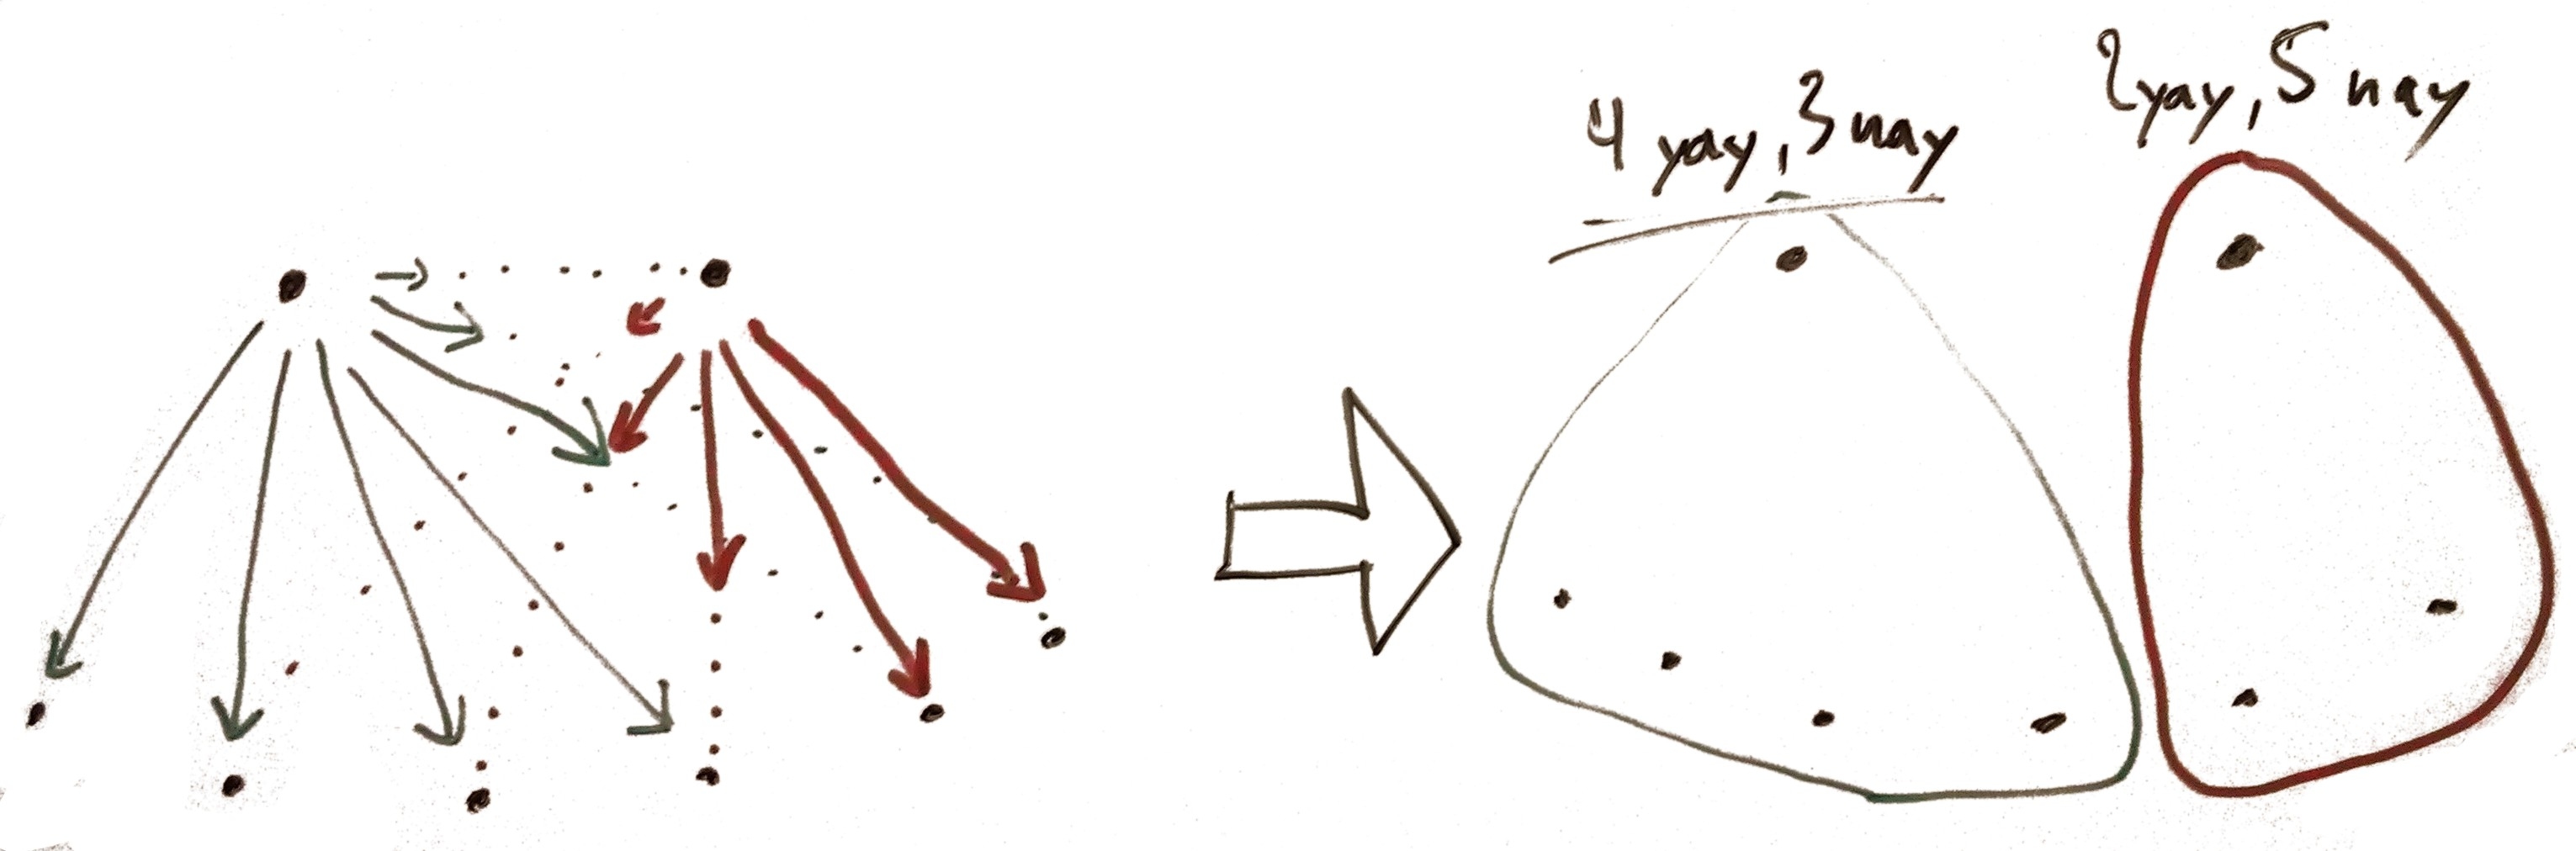
\includegraphics[width=\linewidth]{lock-partition.jpg}
  \caption{Possible partitioning when two nodes try to lock in a chunk swarm}
\end{figure}

All locks are timed to ensure robustness to peer loss. A synchronized clock is
used among the dmap clients.

\subsubsection{Joining a chunk}
See figure \ref{fig:join}.
In order to join a chunk, a client (D) must at least know the address of one of
the chunk participants. That peer, the "adder" (A), locks the chunk such that
the chunk
data is not modified during the process of adding the new peer.

Once the lock is acquired, the adder sends the address of the new peer to the
chunk swarm (B,C), the addresses in the swarm to the new peer, and the chunk 
data to the new peer.

\begin{figure}[H]
  \centering
  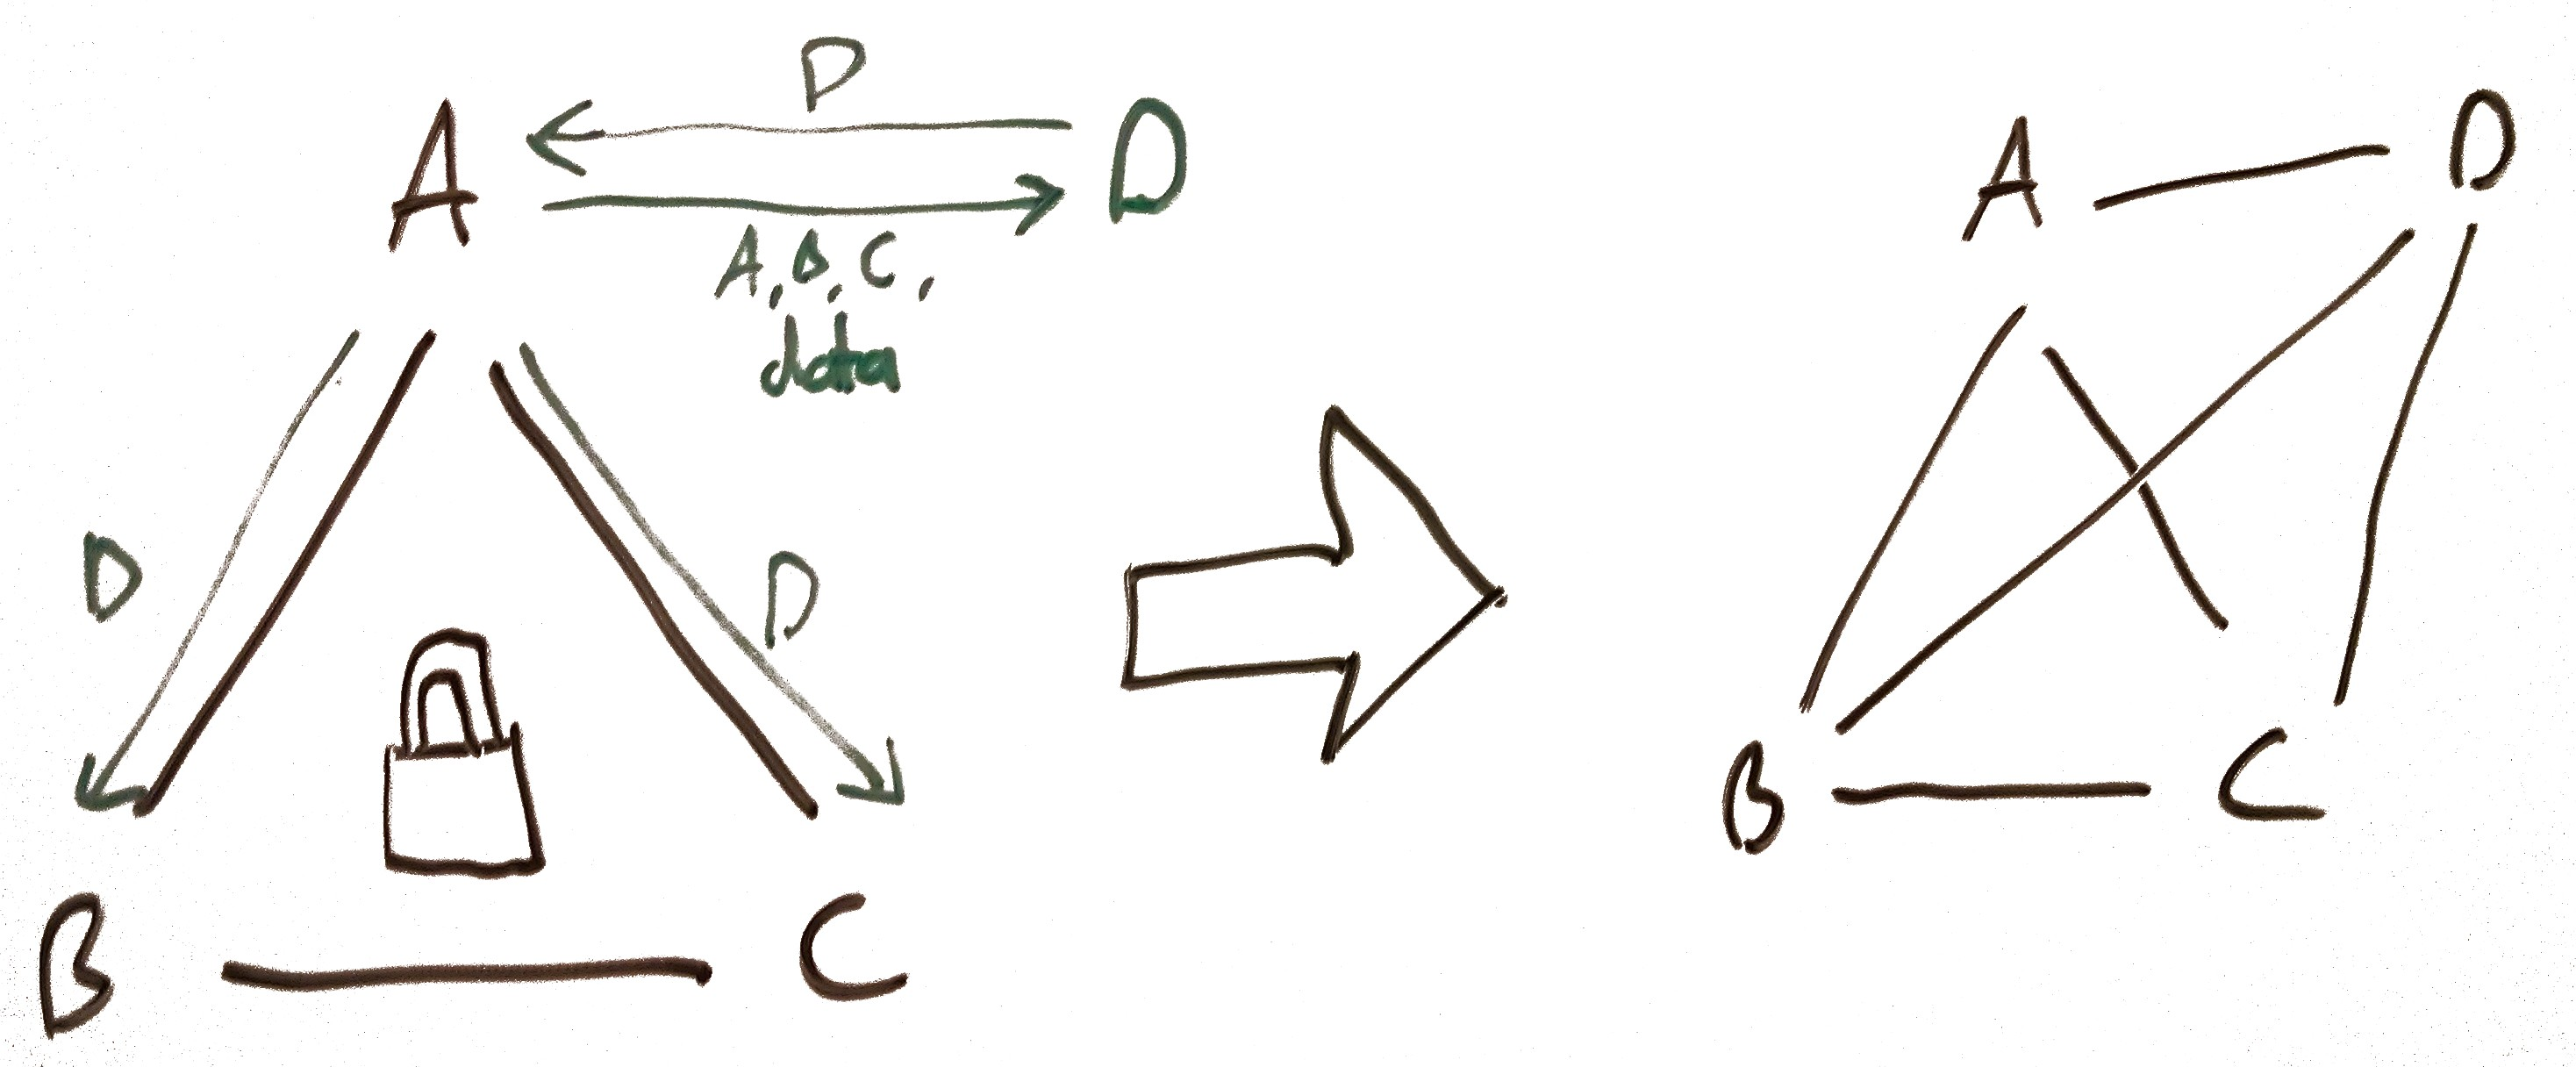
\includegraphics[width=\linewidth]{joining.jpg}
  \caption{Schema of a peer joining a chunk swarm}
  \label{fig:join}
\end{figure}

Locally in the clients, the lock is a reader/writer lock: It is write-locked
for peer addition and read-locked for all other operations.

\subsubsection{Leaving a chunk and robustness to peer loss}

Unlike with joining, locking is not required. There are two ways a peer can leave
the swarm: With or without (swarm-broadcast) notification.

When the peer leaves without notification, the first peer that tries to connect
with it and fails sends out the notification.

Peers in the swarm have the ability to send out chunk participation requests
to table peers (see below), even if the latter don't require access to chunk
data. This gives content creators the ability to ensure that their newly created
content persists in the network even if nobody requests their data before they
leave the network. 

For now, acceptance of participation requests relies on good will, i.e. it is 
not incentivized. It is at this point that irrelevant data gets removed from the
network over time: Peers may decide to impose a limit on chunks held on good
will, and periodically discard least recently accessed chunks, by monitoring
chunk activity.

\subsubsection{Data insertion}

To insert data into a chunk, the peer addition lock must be read-locked, only 
locally. Once that is the case, the inserted data is simply shared with the 
swarm.

\subsubsection{Updates}

To update data, first the local peer addition lock must be read-locked, then a 
distributed update lock must be acquired after which the update is shared with 
the swarm.

\subsubsection{Chunk age}

Because chunk size of updatable table chunks could conceivably grow over time,
we would like to introduce "chunk age": As a peer joins a chunk it may specify
a time (typically "now"). Data that is outdated at that time is then not sent
to the new peer.

\subsection{Table}

Each client holds a peer list for each table that it participates in. Unlike
chunk swarms, table swarms don't need to be fully connected, but, like in
Bitcoin, each client should hold a minimum of connections.

Similarly, each client holds a peer list for the entire dmap, and the
operation for joining tables in the dmap are equivalent to the operations for
joining chunks in a table.

\subsubsection{Naive index lookup}

If a client knows the ID of the table item it is looking for, it sends out a
request to the table swarm. Each peer that receives such a request then looks 
for the data in its instance of the table and either responds with chunk
identifier and its own address or forwards the request to its own peers in
rumor spreading fashion \cite{bitcoin}. While this might result in querying the
entire table swarm with the request, the requester does not need to wait for the
request to traverse the entire network, but only for a first positive response.
Alternatively, $p$ could be assigned such that with probability $p$, each node
receiving the request checks back with the requester whether the request is
still valid.

\subsubsection{K-d tree (binary tree, quadtree, octree) range lookup}

The ID of the item that is looked for is not always known a priori. Sometimes
it is interesting to do lookup in a bounding box. For instance, in robotic
mapping applications it is useful to find other missions that have been recorded
in the same location as an ongoing mission, or to see what part of the
world close to a certain location has not been explored yet.

For such purposes, each table may have one or several k-d tree indices.
The root node of the k-d tree is shared among all table participants. Each
node then holds the peer list of its $2^k$ subnodes unless it is a leaf node,
in which case it holds a list of chunks that have data present in the space
represented by the leaf node.

Nodes in the k-d tree are similar to chunks and tables in terms of networking
responsibilities of their participants. Leaf nodes are considered variable and
are therefore similar to chunks for their update mechanism, while the other
nodes are considered final and can therefore e.g. have not fully connected
swarms. A current disadvantage of that would be that the maximal dimensions of
the data would need to be know in advance.

In order to enforce a healthy amount of peers in the index nodes, peers holding
chunks could be made to hold the corresponding index nodes as well. A peer
holding an index node must also hold all its ancestors.

\section{Ideas for later (not relevant to our questions - feel free to skip)}

\paragraph{Chunk swarm not fully connected}
What would be the implications?

\paragraph{Joining a chunk: Fetching data from multiple peers} 
BitTorrent-style

\paragraph{Disk caching}
Until now, we have implicitly assumed that the table data at the clients sits
in RAM. However, this does not always make sense: Robots might want to store 
data for subsequent offline lookup and volunteer chunk participants might not
want to clutter their RAM with data they don't need anyways. It would thus make
sense to come up with a scheme which decides when to commit data to the disk.

\paragraph{Chunk reactivation}
Disk caching could allow to store data even of inactive chunks. It could happen
that a chunk loses its entire swarm, but then a while later some client would
like to reactivate it again (not necessarily the one holding the data on disk),
because it needs to access the "latest" data again. Such a chunk reactivation
would carry a lot of consequences with it that we haven't thought of yet, but 
the ability to reactivate chunks would probably be very useful.

\begin{thebibliography}{9}
  \bibitem{bitcoin} Decker, C., Wattenhofer, R. (2013, September) 
    \emph{Information propagation in the Bitcoin Network} 
    Peer-to-Peer Computing (P2P), 2013 IEEE Thirteenth International Conference
    on (pp. 1-10). IEEE.
  \bibitem{freenet} Clarke, I., Sandberg, O., Wiley, B., Hong, T. W. 
    (2001, January). \emph{Freenet: A distributed anonymous information storage
    and retrieval system} Designing Privacy Enhancing Technologies (pp. 46-66).
    Springer Berlin Heidelberg.
  \bibitem{discovery} 
    https://en.bitcoin.it/wiki/Satoshi\_Client\_Node\_Discovery
\end{thebibliography}

\end{document}
